\documentclass{beamer}

% You can uncomment the themes below if you would like to use a different
% one:
%\usetheme{AnnArbor}
%\usetheme{Antibes}
%\usetheme{Bergen}
%\usetheme{Berkeley}
%\usetheme{Berlin}
%\usetheme{Boadilla}
\usetheme{Frankfurt}
%\usetheme{boxes}
%\usetheme{CambridgeUS}
%\usetheme{Copenhagen}
%\usetheme{Darmstadt}

%CREATES THE TABLE OF CONTENTS AT THE TOP
%\useoutertheme[subsection=false,shadow]{miniframes}
%\useinnertheme{default}
\usepackage{tikz}
\usepackage{listings}
\usetikzlibrary{shapes.geometric, arrows, positioning, calc}
\tikzstyle{startStop} = [rectangle, rounded corners, minimum width=7cm, text width=11cm, text centered, minimum height=.5cm, draw=black]
\tikzstyle{io} = [circle, rounded corners, minimum width=1cm, text width=1.5cm, minimum height=.1, text centered, draw=black]
\tikzstyle{arrow} = [thick,->,>=stealth]
\usepackage{pdfpages}
\usepackage{graphicx}   % need for figures
\usepackage{adjustbox}
\usepackage{fontawesome}
\usepackage[absolute,overlay]{textpos}
%CHANGES COLOR TO GREEN
\usepackage{listings} 
\usepackage{color}
 
\definecolor{codegreen}{rgb}{0,0.6,0}
\definecolor{codegray}{rgb}{0.5,0.5,0.5}
\definecolor{codepurple}{rgb}{0.58,0,0.82}
\definecolor{backcolour}{rgb}{0.95,0.95,0.92}
 
\lstdefinestyle{mystyle}{
    backgroundcolor=\color{backcolour},   
    commentstyle=\color{codegreen},
    keywordstyle=\color{magenta},
    numberstyle=\tiny\color{codegray},
    stringstyle=\color{codepurple},
    basicstyle=\scriptsize,
    breakatwhitespace=true,         
    breaklines=true,                 
    captionpos=b,                    
    keepspaces=false,                 
    numbers=left,                    
    numbersep=5pt,                  
    showspaces=false,                
    showstringspaces=false,
    showtabs=false,                  
    tabsize=2
}
 
\lstset{style=mystyle}
\definecolor{brickred}{rgb}{0.8, 0.25, 0.33}
\definecolor{mygreen}{cmyk}{0.82,0.11,1,0.25}
\setbeamertemplate{blocks}[rounded][shadow=true]
\addtobeamertemplate{block begin}{\pgfsetfillopacity{0.8}}{\pgfsetfillopacity{1}}
\setbeamercolor{structure}{fg=mygreen}
\setbeamercolor*{block title example}{fg=white,
bg= white}
\setbeamercolor*{block body example}{fg= white,
bg= white}
\usepackage[english]{babel}
\usepackage{hyperref}
\usepackage{dcolumn}
\usepackage{adjustbox}
\usepackage{multicol}
\usepackage{adjustbox}
\usepackage{amsmath}
\usepackage{tikz}
\usepackage[all,cmtip]{xy}
\tikzstyle{largeSquare} = [rectangle, rounded corners, minimum width=7cm, text width=9cm, minimum height=.5cm, draw=black]

\usetikzlibrary{shapes.geometric, arrows}
\tikzstyle{arrow}=[thick,->,>=stealth]
\beamertemplatenavigationsymbolsempty
\usepackage{subfloat}
\setbeamertemplate{headline}{}
\newcommand{\speechthis}[2]{
        \tikz[remember picture,baseline]{\node[anchor=base,inner sep=0,outer sep=0]%
        (#1) {\underline{#1}};\node[overlay,ellipse callout,fill=blue!50] 
        at ($(#1.north)+(-.5cm,0.8cm)$) {#2};}%
    }%
%\usetheme{Goettingen}
%\usetheme{Hannover}
%\usetheme{Ilmenau}
%\usetheme{JuanLesPins}
%\usetheme{Luebeck}
%\usetheme{Madrid}
%\usetheme{Malmoe}
%\usetheme{Marburg}
%\usetheme{Montpellier}
%\usetheme{PaloAlto}
%\usetheme{Pittsburgh}
%\usetheme{Rochester}
%\usetheme{Singapore}
%\usetheme{Szeged}
%\usetheme{Warsaw}
\setbeamercolor{button}{bg=mygreen,fg=white}
\setbeamercovered{transparent=25}
\usecolortheme{beaver}

\title{Network Analysis: }

\subtitle{Bilateral Investment Treaty Violations}

\author{Jeffrey Ziegler}
\institute{Washington University in St. Louis}

\date{\today}

\usepackage[framemethod=tikz]{mdframed}

\begin{document}

{ \usebackgroundtemplate{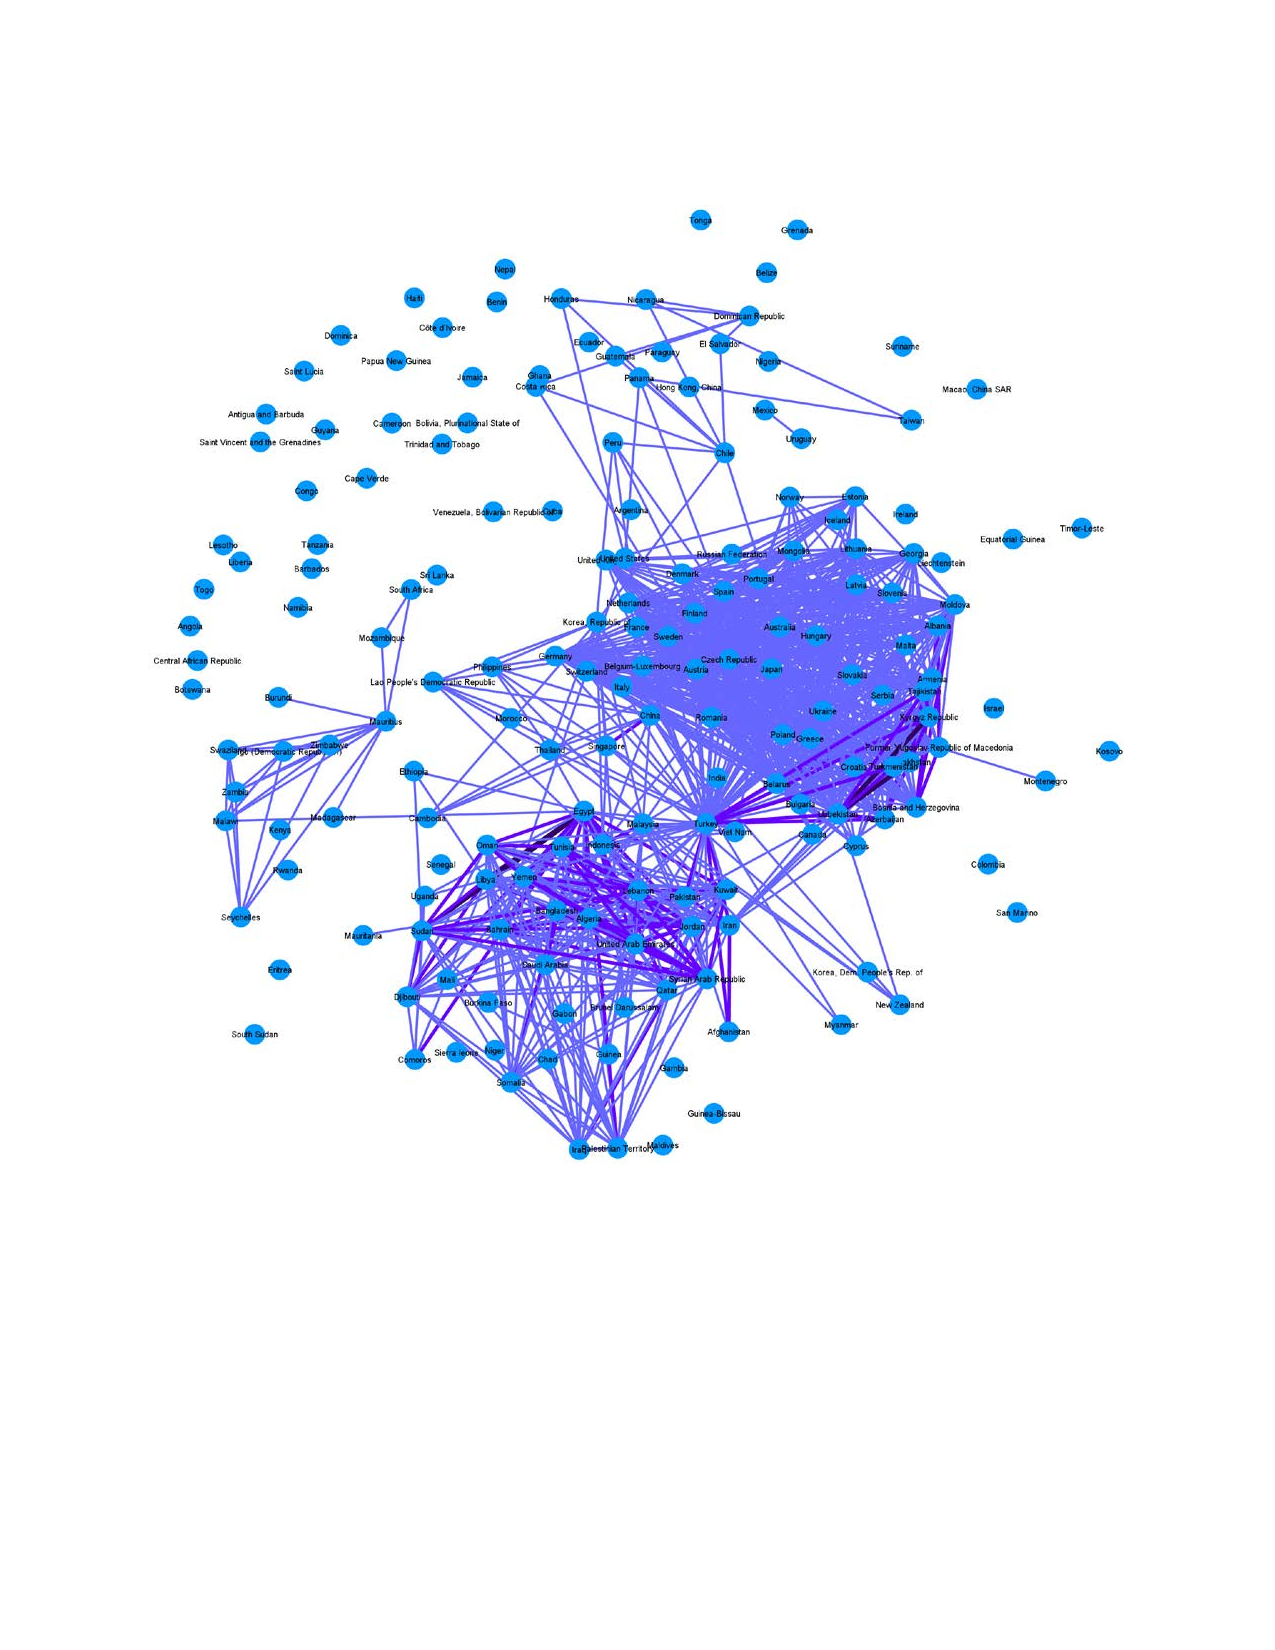
\includegraphics[width=.8\paperwidth, height=1\paperheight]{figures/background.pdf}}
  \begin{frame}[plain]
\begin{centering}
\begin{mdframed}[tikzsetting={draw=gray,fill=white,fill opacity=0.8,
               line width=1pt},backgroundcolor=none,leftmargin=2,
               rightmargin=2, innertopmargin=8pt]
\Large{\inserttitle}\\
\large{\insertsubtitle}\\ \\
\insertauthor, \insertinstitute
\end{mdframed}
\end{centering}
\vspace{5em}
\begin{mdframed}[tikzsetting={draw=gray,fill=white,fill opacity=0.8,
               line width=1pt},backgroundcolor=none, leftmargin=140,
               rightmargin=0, innertopmargin=8pt]
 \faEnvelope \ \href{mailto:jeffreyziegler@wustl.edu} {\tt jeffreyziegler@wustl.edu}\\
    \faHome \ \href{https://zieglerjef.github.io/} {\tt jeffreyziegler.org} \\
    \faGithub \ \href{https://github.com/zieglerjef} {\tt zieglerjef}
\end{mdframed}
\end{frame}
}

\begin{frame}[fragile]{\large Investment treaty data: Basic overview.}
\begin{lstlisting}[language=R]
# show biggest "suers" (origin country of plantiff)
head(sort(rowSums(BITadjMatTotalMatrix), decreasing = T))
# show biggest violators (countries that pass potentially expropriating policies)
head(sort(colSums(BITadjMatTotalMatrix), decreasing = T))
\end{lstlisting}

\begin{verbatim}
United States United Kingdom  Spain Venezuela Italy Turkey 
38             30             15    13        12    10 

Argentina Netherlands Ecuador Germany Czechslovakia Italy 
33        13          12      11      10            10
\end{verbatim}
\end{frame}

\begin{frame}{\large Empirically, democracies sign and violate, investment treaties more frequently (and importantly, more disproportionately).}

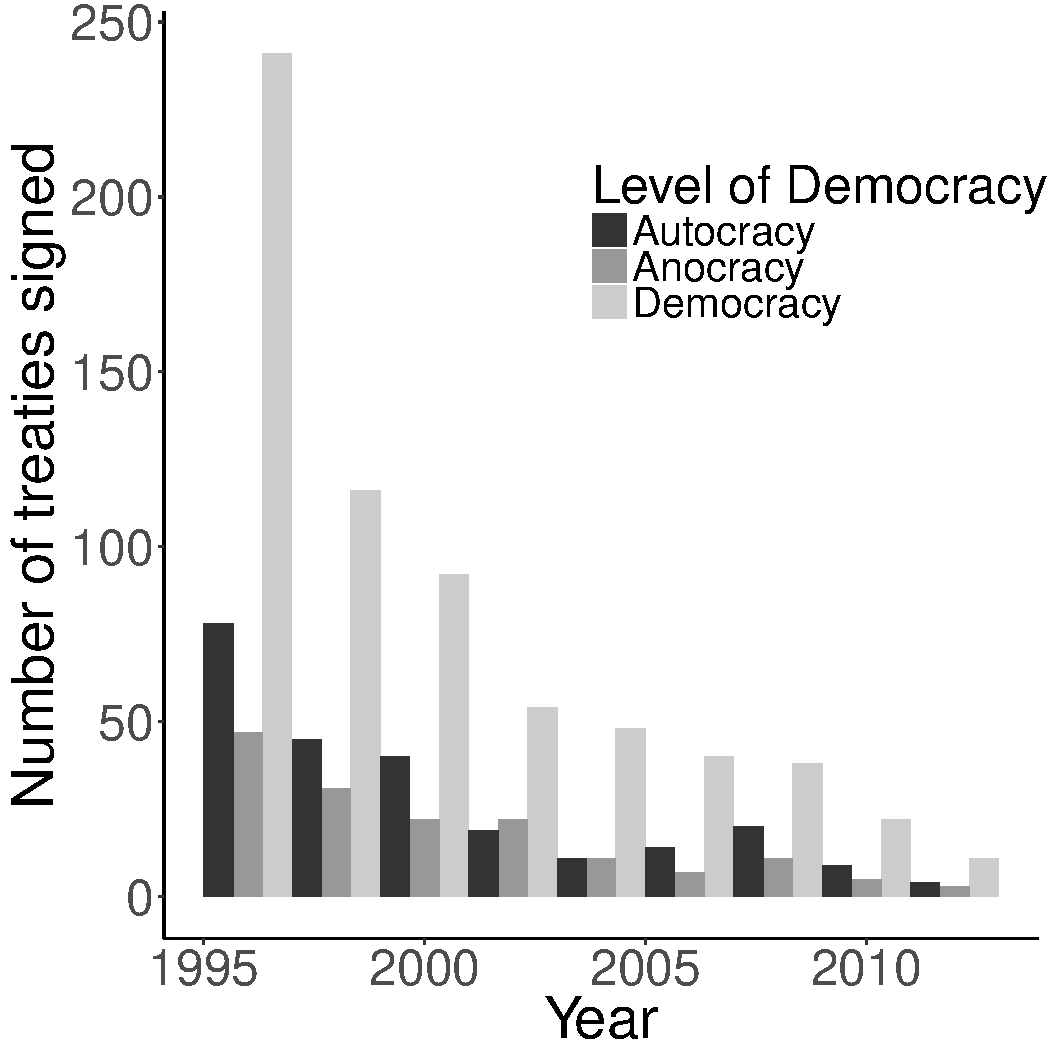
\includegraphics[width=.49\linewidth]{figures/histSignRegimeType.pdf}
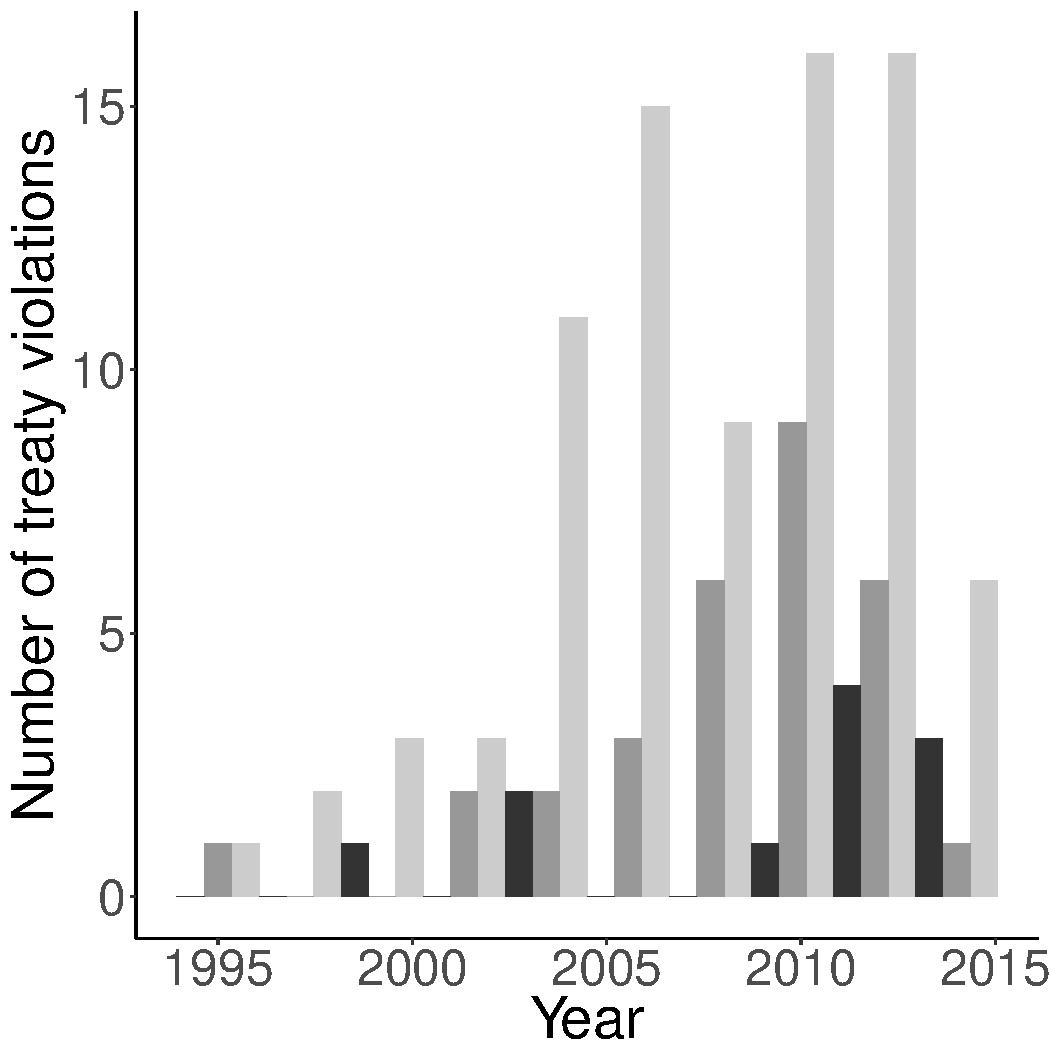
\includegraphics[width=.49\linewidth]{figures/histViolationRegimeType.pdf}

\begin{center}
	{\Large Puzzle: Why?}
\end{center}
\end{frame}


\begin{frame}{\large If elections are what make democracies democratic, and democracies are good treaty partners, then lack of elections should increase violations?}

\setbeamercovered{invisible}
\begin{center}
	\pause
	{\Large NO!}
\end{center}
\end{frame}

\begin{frame}{\large Governments, in general, are more likely to pass expropriating policies (i.e. violate BIT) when they soon face credible elections.}

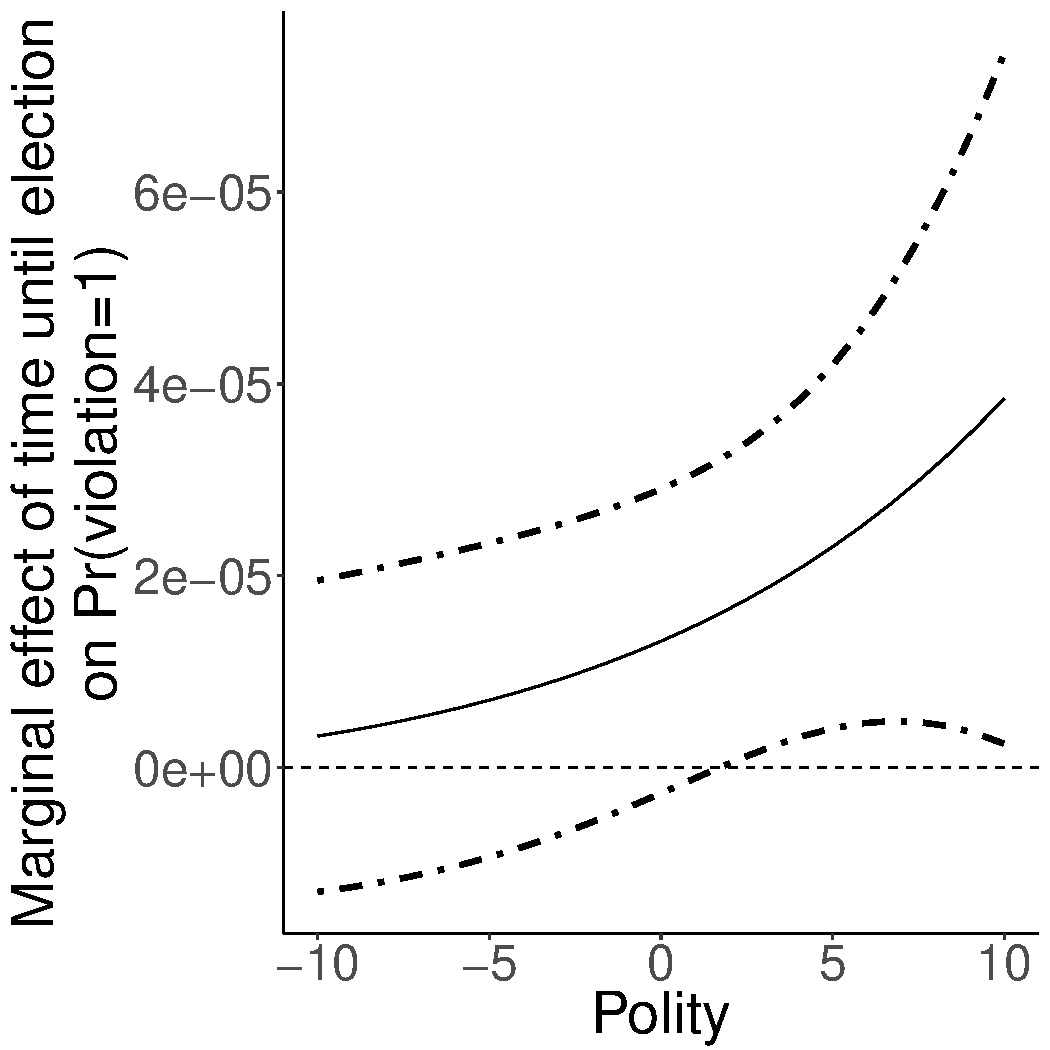
\includegraphics[width=.49\linewidth]{figures/polity2Effect.pdf}
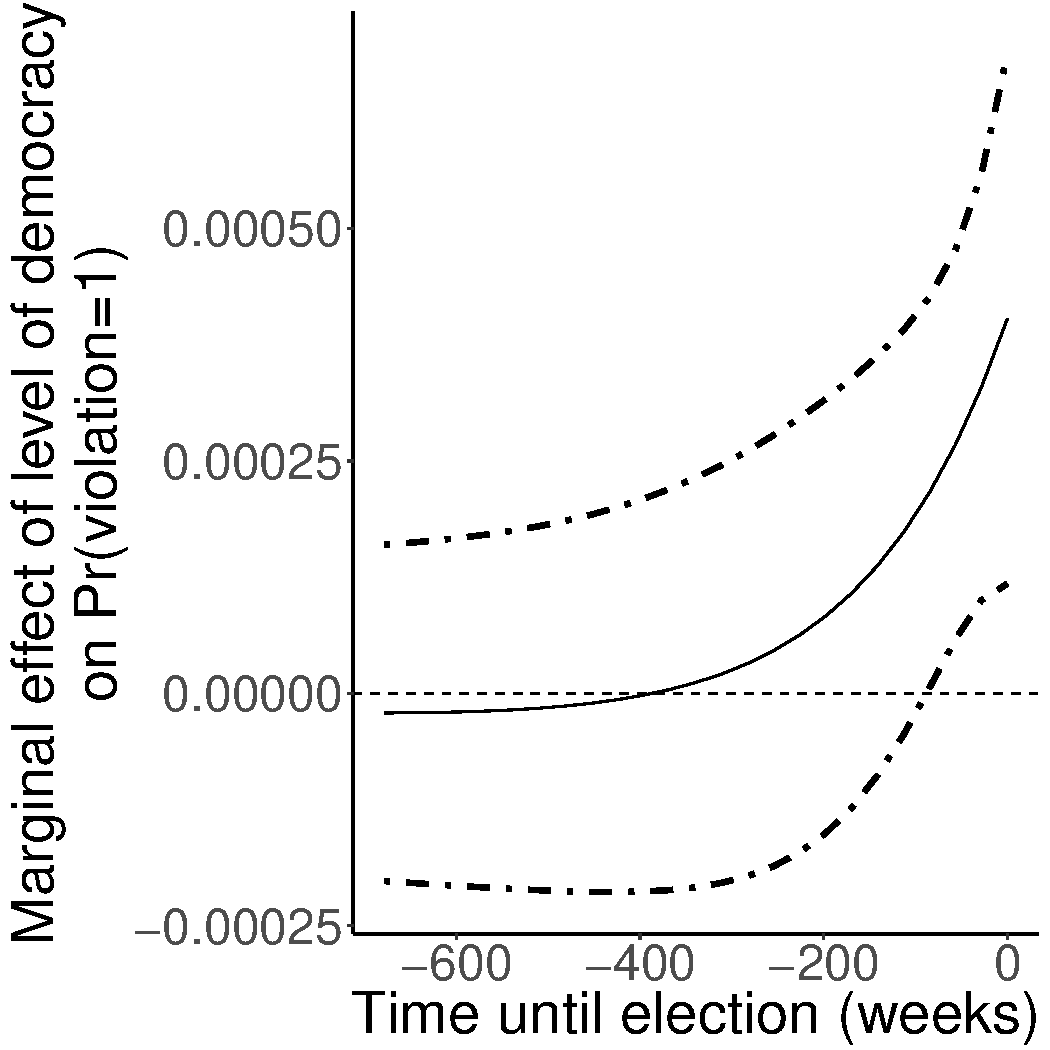
\includegraphics[width=.49\linewidth]{figures/timeUntilAnyElecEffect.pdf}

\setbeamercovered{invisible}
\begin{center}
	\pause
	{Maybe arbitration timing is strategic (i.e. as $t \rightarrow$ elections), and litigation is driven by the relationship between the two countries involved in the treaty?}
\end{center}
\end{frame}

\begin{frame}[fragile]{\large Investment treaty network: Network overview.}

\begin{lstlisting}[language=R]
# check proportion of present edges from all possible edges in the network.
# for a directed network
ecount(yGraph)/(vcount(yGraph)*(vcount(yGraph)-1))
# very little violations in general, so unsuprising
\end{lstlisting}
\begin{verbatim}
[1] 0.01820728
\end{verbatim}

\begin{lstlisting}[language=R]
reciprocity(yGraph)
# doesn't seem like passing expropriating policies
# leads to other countries to sue, and then pass expropriating policies
\end{lstlisting}
\begin{verbatim}
[1] 0
\end{verbatim}
\end{frame}

\begin{frame}{\large Investment treaty network: Latent Distance Model.}

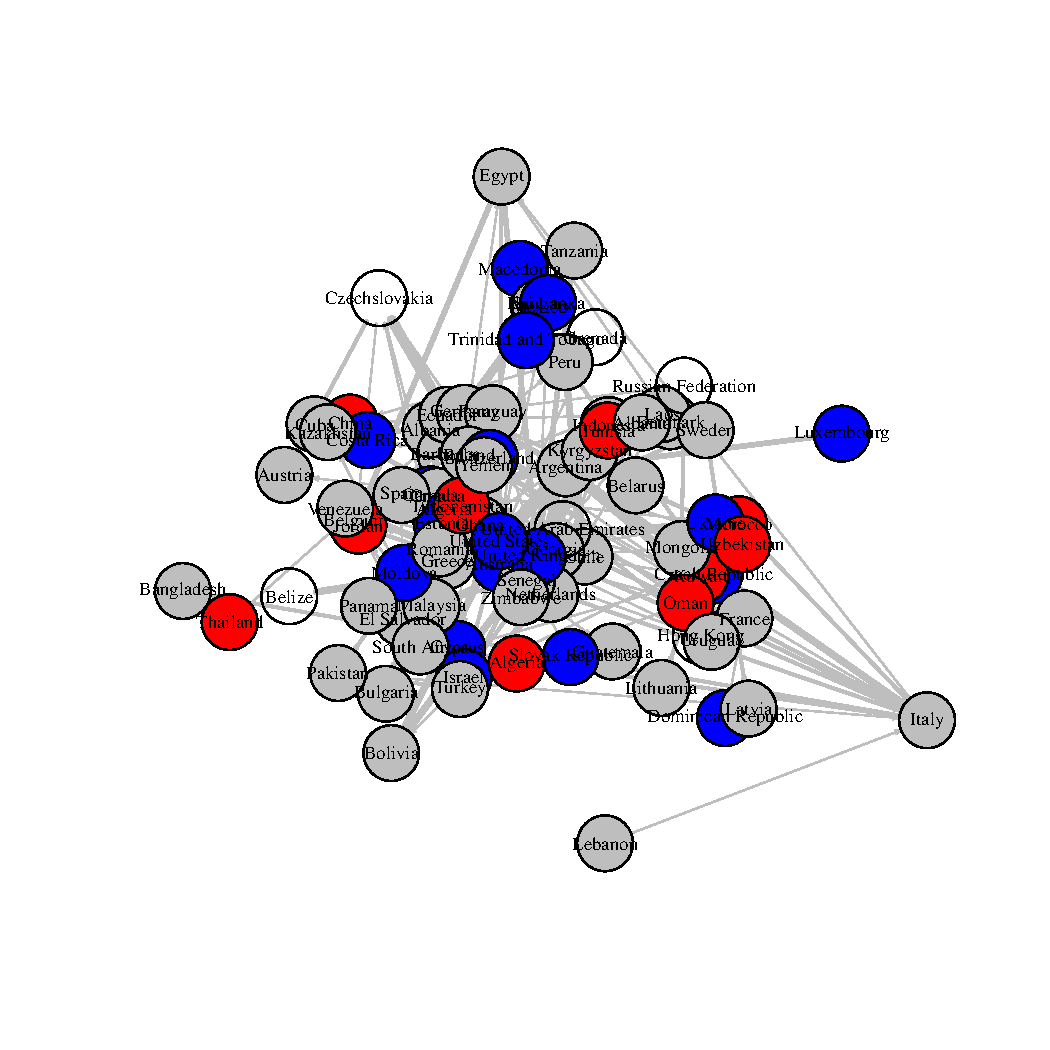
\includegraphics[width=.99\linewidth]{../figure3.pdf}
\end{frame}

\end{document}